\documentclass[letterpaper,MMMyyyy,nonstopmode]{resumecv}
% Class options:
% a4paper, letterpaper, nonstopmode, draftmode
% MMMyyyy, ddMMMyyyy, MMMMyyyy, ddMMMMyyyy, yyyyMMdd, yyyyMM, yyyy

\usepackage{eso-pic,graphicx}
\usepackage{xcolor}
\usepackage{adjustbox}
%%%%%%%%%%%%%%%%%%%%%%%%%%%%%%%%%%%%%%%%%%%%%%%%%%%%%%%%%%%%%%%%%
%% PREAMBLE.
%%%%%%%%%%%%%%%%%%%%%%%%%%%%%%%%%%%%%%%%%%%%%%%%%%%%%%%%%%%%%%%%%

% CV Info (to be customized).
\newcommand{\CVAuthor}{Marcos Quezada Pérez}
\newcommand{\CVTitle}{John Doe's CV for Acme Corporation}
\newcommand{\CVNote}{CV compiled on {\today} for Acme Corporation}
\newcommand{\CVWebpage}{http://www.example.com/~johndoe}

% PDF settings and properties.
\hypersetup{
pdftitle={\CVTitle},
pdfauthor={\CVAuthor},
pdfsubject={\CVWebpage},
pdfcreator={XeLaTeX},
pdfproducer={},
pdfkeywords={},
unicode=true,
bookmarks=true,
bookmarksopen=true,
pdfstartview=FitH,
pdfpagelayout=OneColumn,
pdfpagemode=UseOutlines,
hidelinks,
breaklinks}

% Shorthand.
\newcommand{\Code}[1]{\mbox{\textbf{#1}}}
\newcommand{\CodeCommand}[1]{\mbox{\textbf{\textbackslash{#1}}}}

%%%%%%%%%%%%%%%%%%%%%%%%%%%%%%%%%%%%%%%%%%%%%%%%%%%%%%%%%%%%%%%%%
%% ACTUAL DOCUMENT.
%%%%%%%%%%%%%%%%%%%%%%%%%%%%%%%%%%%%%%%%%%%%%%%%%%%%%%%%%%%%%%%%%

\begin{document}

\AddToShipoutPictureBG{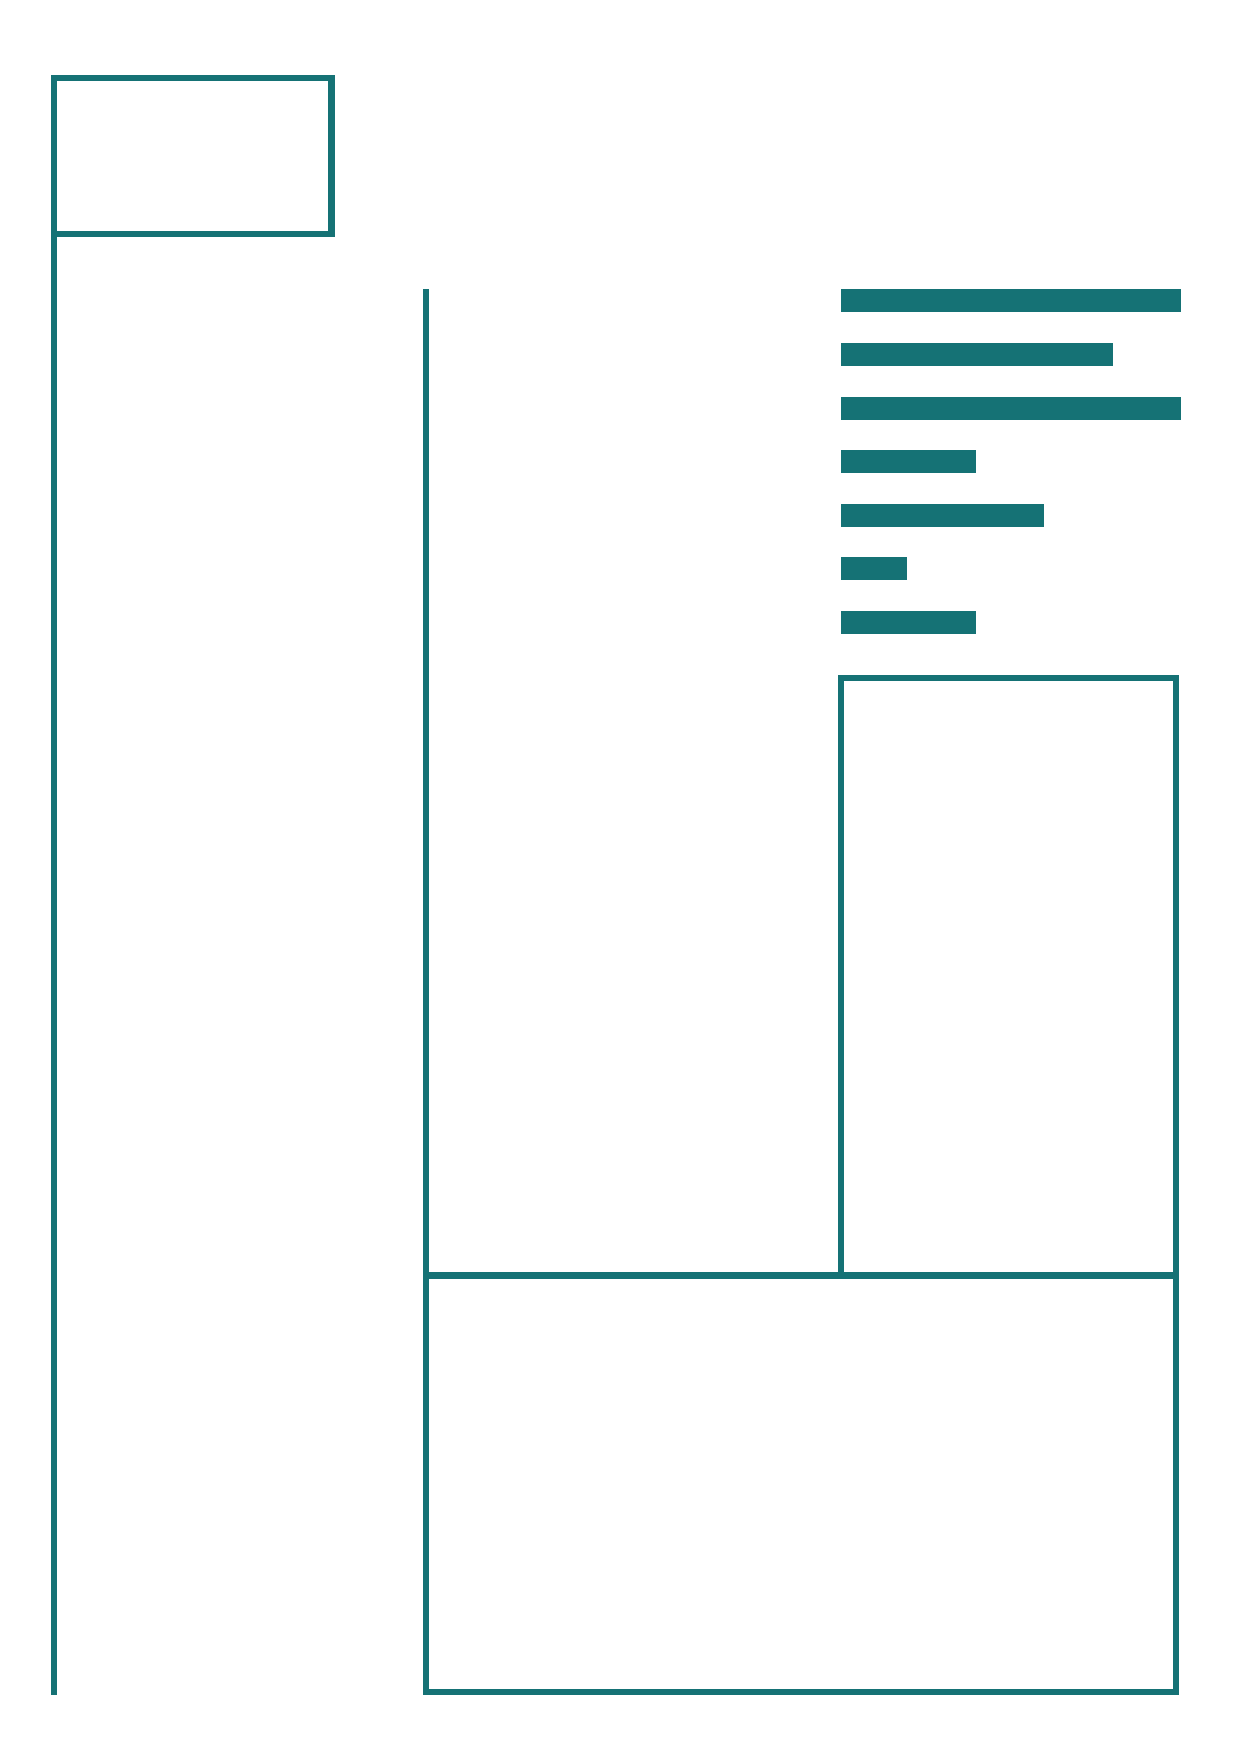
\includegraphics[width=\paperwidth,height=\paperheight]{page1.png}}

%%%%%%%%%%%%%%%
% TITLE BLOCK %
%%%%%%%%%%%%%%%

\begin{adjustbox}{minipage=0.25\textwidth-2\fboxsep-2\fboxrule,cfbox=teal 2pt}\UseTitleFont
\href{https://www.google.com/maps/place/17+Prime+Avenue,+Springfield,+Pennsylvania+10111,+USA}
{17 Prime Avenue, Apt 37, Springfield, Pennsylvania 10111, USA}
\par
\href{mailto:johndoe@example.com}
{johndoe@example.com}
\,\SubBulletSymbol\,
+1\,(555)\,101-1001
\,\SubBulletSymbol\,
\href{\CVWebpage}
{\url{\CVWebpage}}
\end{adjustbox}
\hfill{\color{teal}\vline width 2pt}\hfill
\begin{fmpage}{0.70\textwidth\raggedleft\UseTitleFont}\raggedleft
\CVAuthor
\end{fmpage}


\begin{Title}{\CVAuthor}\raggedleft
\end{Title}

\begin{SubTitle}\raggedright
\href{https://www.google.com/maps/place/17+Prime+Avenue,+Springfield,+Pennsylvania+10111,+USA}
{17 Prime Avenue, Apt 37, Springfield, Pennsylvania 10111, USA}
\par
\href{mailto:johndoe@example.com}
{johndoe@example.com}
\,\SubBulletSymbol\,
+1\,(555)\,101-1001
\,\SubBulletSymbol\,
\href{\CVWebpage}
{\url{\CVWebpage}}
\end{SubTitle}

\begin{Body}

%%%%%%%%%%%%%%%
%% EDUCATION %%
%%%%%%%%%%%%%%%

\Section
{Education}
{Education}
{PDF:Education}

\Entry
\href{http://www.example.com/my-university}
{\textbf{First American University}},
Springfield, Massachusetts, USA

\Gap
\BulletItem
Ph.D. in
\href{http://www.example.com/my-department}
{Geophysical Engineering}
\hfill
\DatestampYMD{2009}{12}{15} --
\DatestampYMD{2014}{07}{15}
\begin{Detail}
\SubBulletItem
Thesis:
\href{http://www.example.com/my-phd-thesis}
{A Statistical Approach to Quantifying Climate Change}
\SubBulletItem
Adviser:
Prof.~Jonathan~Public
\SubBulletItem
Focus:
Climate change, metrology, lasers, statistics.
\end{Detail}

\Gap
\BulletItem
M.B.A.
\hfill
\DatestampYMD{2008}{11}{15} --
\DatestampYMD{2009}{06}{15}

\Gap
\BulletItem
M.S. in
\href{http://www.example.com/my-department}
{Geophysical Engineering}
\hfill
\DatestampYMD{2006}{08}{15} --
\DatestampYMD{2008}{08}{15}
\begin{Detail}
\SubBulletItem
Cumulative GPA: 3.7 / 4.0
\end{Detail}

\BigGap
\Entry
\href{http://www.example.com/my-college}
{\textbf{Science College}},
Springfield, Pennsylvania, USA

\Gap
\BulletItem
B.S. in
\href{http://www.example.com/my-department}
{Geography}
\hfill
\DatestampYMD{2002}{05}{15} --
\DatestampYMD{2005}{05}{15}
\begin{Detail}
\SubBulletItem
Graduated with College Honors.
\SubBulletItem
Cumulative GPA: 3.96 / 4.00
\end{Detail}

%%%%%%%%%%%%%%%%%%%%%%%%%
%% RESEARCH EXPERIENCE %%
%%%%%%%%%%%%%%%%%%%%%%%%%

\Section
{Research Experience}
{Research Experience}
{PDF:ResearchExperience}

\Entry
\href{http://www.example.com/my-institute}
{\textbf{Institute for Advanced Research}},
Science College

\Gap
\BulletItem
Undergraduate Research Student, Science Department
\hfill
\DatestampYMD{2004}{05}{15} --
\DatestampYMD{2005}{05}{15}
\begin{Detail}
\SubBulletItem
Project:
Investigations on the Use of Lasers to Measure Climate Change
\SubBulletItem
Supervisors:
Prof.~Jane~Citizen and
Dr~Ann~Yone
\SubBulletItem
Focus:
Climate change, lasers, statistical analysis, data analytics.
\end{Detail}

%%%%%%%%%%%%%%%%%%
%% PUBLICATIONS %%
%%%%%%%%%%%%%%%%%%

\Section
{Publications}
{Publications}
{PDF:Publications}

\SubSection
{Journals}
{Journals}
{PDF:Journals}

% Declare a new group to limit the scope of \MaxNumberedItem to this subsection.
\begingroup
\renewcommand{\MaxNumberedItem}{[88]}

\BigGap
\NumberedItem{[10]}
\href{http://www.example.com/my-paper-doi-5}
{\underline{J.~Doe}, J.~Citizen, and A.~Yone,
``On lasers and climate change,''
\textit{Journal of Science},
vol.~89,
no.~2,
pp.~4123--4133,
\DatestampYM{2008}{02}.}

\Gap
\NumberedItem{[1]}
\href{http://www.example.com/my-paper-doi-4}
{\underline{J.~Doe} and J.~Citizen,
``Measuring the extent of climate change,''
\textit{Global Scientific Journal},
vol.~12,
no.~4,
pp.~330--352,
\DatestampYM{2006}{12}.}

\endgroup

\BigGap
\SubSection
{Conferences}
{Conferences}
{PDF:Conferences}

% Declare a new group to limit the scope of \MaxNumberedItem to this subsection.
\begingroup
\renewcommand{\MaxNumberedItem}{[8888]}

\BigGap
\NumberedItem{[1000]}
\href{http://www.example.com/my-paper-doi-3}
{\underline{J.~Doe}, J.~Citizen, and A.~Yone,
``On lasers and climate change,''
in \textit{Proceedings of the Laser Symposium},
Las Vegas, Nevada, USA,
\DatestampYM{2007}{01}.}

\Gap
\NumberedItem{[100]}
\href{http://www.example.com/my-paper-doi-2}
{A.~Yone and \underline{J.~Doe},
``Climate change and general relativity,''
in \textit{Proceedings of the International Astronomical Conference},
Sydney, Australia,
\DatestampYM{2006}{8}.}

\Gap
\NumberedItem{[10]}
\href{http://www.example.com/my-paper-doi-1}
{\underline{J.~Doe} and J.~Citizen,
``Measuring the extent of climate change,''
in \textit{Proceedings of the International Climate Change Conference},
London, UK,
\DatestampYM{2005}{11}.}

\endgroup

%%%%%%%%%%%%%%%%%%%%%%%%%%%
%% AWARDS & SCHOLARSHIPS %%
%%%%%%%%%%%%%%%%%%%%%%%%%%%

\Section
{Awards \&\newline
Scholarships}
{Awards \& Scholarships}
{PDF:AwardsAndScholarships}

\BulletItem
Dean's List,
Fall 2002 through Spring 2005,
Science College
\hfill
\DatestampY{2002} --
\DatestampY{2005}
\begin{Detail}
\Item
For attaining a semester GPA of at least 3.75.
\end{Detail}

\Gap
\BulletItem
Undergraduate Researcher Award,
Science College
\hfill
\DatestampYMD{2005}{05}{15}
\begin{Detail}
\Item
For outstanding scientific contributions in the fields of lasers and climate change.
\end{Detail}

\Gap
\BulletItem
Chess Tournament,
First Prize,
Science College
\hfill
\DatestampYMD{2003}{03}{10}
\begin{Detail}
\Item
Awarded at the Tenth Annual Chess Tournament held during Open House.
\end{Detail}

\Gap
\BulletItem
International Science Scholarship,
\hfill
\DatestampYMD{2001}{12}{10}
\newline
Global Science, Technology, Engineering, and Mathematics Foundation
\begin{Detail}
\Item
Full-tuition scholarship with stipend for undergraduate studies.
One of 42 awardees in the world.
\end{Detail}

%%%%%%%%%%%%%%%%%%%%%%%%%%%%%%%%%%%%%%%%%%%%
%% PROFESSIONAL AFFILIATIONS & ACTIVITIES %%
%%%%%%%%%%%%%%%%%%%%%%%%%%%%%%%%%%%%%%%%%%%%

\Section
{Professional Affiliations\newline
\& Activities}
{Professional Affiliations \& Activities}
{PDF:ProfessionalAffiliationsActivities}

\Entry
\href{http://www.example.com/my-society}
{\textbf{Joint Society of Earth Scientists and Global Think Tank on Climate Resiliency}},
\newline
North Attleborough, Massachusetts, USA

\Gap
\BulletItem
Member
\hfill
\DatestampY{2009} --
Present

% Manual page break.
\newpage

%%%%%%%%%%%%%%%%%%%%%%%
%% CAMPUS ACTIVITIES %%
%%%%%%%%%%%%%%%%%%%%%%%

\Section
{Campus Activities}
{Campus Activities}
{PDF:CampusActivities}

\Entry
\href{http://www.example.com/my-club}
{\textbf{First Volunteers Club}},
First American University

\Gap
\BulletItem
President
\hfill
\DatestampYMD{2006}{08}{15} --
\DatestampYMD{2007}{08}{15}
\begin{Detail}
\SubBulletItem
Lorem ipsum dolor sit amet, consectetur adipiscing elit.
\SubBulletItem
Curabitur vitae laoreet velit, vel ultricies est. Nam nec elit ac ante facilisis ultrices.
\SubSubBulletItem
Wel turpis efficitur, non lacinia orci maximus.
\SubSubBulletItem
Proin rhoncus, felis vel hendrerit lacinia.
\SubBulletItem
Integer sit amet turpis dolor. Lorem ipsum dolor sit amet, consectetur adipiscing elit. Nunc at orci eu leo vulputate finibus sed et sem.
\SubBulletItem
Suspendisse volutpat sapien et mi cursus, gravida ornare mauris sollicitudin.
\end{Detail}

%%%%%%%%%%%%%%%%%%%%%%%%%%%
%% OTHER WORK EXPERIENCE %%
%%%%%%%%%%%%%%%%%%%%%%%%%%%

\Section
{Other Work\newline
Experience}
{Other Work Experience}
{PDF:OtherWorkExperience}

\Entry
\href{http://www.example.com/my-company}
{\textbf{Alpha Engineering Firm}},
Oakland, Ohio, USA

\Gap
\BulletItem
Project Officer,
Department of Meteorological Sciences,
\hfill
\DatestampYMD{2007}{10}{15} --
\DatestampYMD{2008}{01}{15}
\newline
Research \& Development Division
\begin{Detail}
\SubBulletItem
Nullam venenatis egestas nisl eget elementum.
\SubBulletItem
Nulla finibus justo vel turpis efficitur, non lacinia orci maximus. Proin rhoncus, felis vel hendrerit lacinia, enim ipsum ultricies massa, sit amet interdum nisi massa sit amet justo.
\SubBulletItem
Etiam vitae eros mollis, consectetur quam quis, molestie massa.
\end{Detail}

%%%%%%%%%%%%%%%
%% LANGUAGES %%
%%%%%%%%%%%%%%%

\Section
{Languages}
{Languages}
{PDF:Languages}

\BulletItem
English: Native language.

\Gap
\BulletItem
Spanish: Fluent (speaking, reading, writing).

\Gap
\BulletItem
Latin: Intermediate (reading); basic (speaking, writing).

%%%%%%%%%%%%
%% SKILLS %%
%%%%%%%%%%%%

\Section
{Skills}
{Skills}
{PDF:Skills}

\Entry
{\TeX}, {\LaTeX}, {\XeLaTeX},
MATLAB,
Mathematica,
Maple,
R,
Tableau,
Adobe Photoshop,
Adobe Illustrator,
Microsoft Word,
Microsoft Excel,
Microsoft PowerPoint.

%%%%%%%%%%%%%%%
%% INTERESTS %%
%%%%%%%%%%%%%%%

\Section
{Interests}
{Interests}
{PDF:Interests}

\Entry
Digital photography,
typography,
swimming.

%%%%%%%%%%%%%%%%
%% REFERENCES %%
%%%%%%%%%%%%%%%%

\Section
{References}
{References}
{PDF:References}

\BulletItem
\textbf{Professor Jonathan Public}
\newline
Professor of Geology and Mechanical Engineering
\newline
First American University
\newline
1000 First Avenue, Springfield, Massachusetts 22222, USA
\newline
\href{mailto:jonathanpublic@example.com}
{jonathanpublic@example.com}
\,\SubBulletSymbol\,
+1\,(555)\,222-2222

\BigGap
\BulletItem
\textbf{Dr Alice Bob Carol}
\newline
Director, Research \& Development
\newline
Alpha Engineering Firm
\newline
20 North Street, Oakland, Ohio 33333, USA
\newline
\href{mailto:alicebobcarol@example.com}
{alicebobcarol@example.com}
\,\SubBulletSymbol\,
+1\,(555)\,333-3333

%%%%%%%%%%%%%%%%%%%%%%%%%%%%%%%%%%%
%% MULTILINGUAL UNICODE EXAMPLES %%
%%%%%%%%%%%%%%%%%%%%%%%%%%%%%%%%%%%

\Section
{Multilingual Unicode Examples}
{Multilingual Unicode Examples}
{PDF:MultilingualUnicodeExamples}

\BulletItem
Assortment of unicode characters from
\href{http://www.ltg.ed.ac.uk/~richard/unicode-sample.html}
{\url{http://www.ltg.ed.ac.uk/~richard/unicode-sample.html}}

\begin{Detail}
\Item
\textbf{Latin Extended-A}
Ā ā Ă ă Ą ą Ć ć Ĉ ĉ Ċ ċ Č č Ď ď Đ đ Ē ē Ĕ ĕ Ė ė Ę ę Ě ě Ĝ ĝ Ğ ğ Ġ ġ Ģ ģ Ĥ ĥ Ħ ħ Ĩ ĩ Ī ī Ĭ ĭ Į į İ ı IJ ij Ĵ ĵ
\textbf{Latin Extended-B}
ƀ Ɓ Ƃ ƃ Ƅ ƅ Ɔ Ƈ ƈ Ɖ Ɗ Ƌ ƌ ƍ Ǝ Ə Ɛ Ƒ ƒ Ɠ Ɣ ƕ Ɩ Ɨ Ƙ ƙ ƚ ƛ Ɯ Ɲ ƞ Ɵ Ơ ơ Ƣ ƣ Ƥ ƥ Ʀ Ƨ ƨ Ʃ ƪ ƫ Ƭ ƭ Ʈ Ư ư Ʊ Ʋ Ƴ ƴ Ƶ
\textbf{Latin Extended Additional}
Ḁ ḁ Ḃ ḃ Ḅ ḅ Ḇ ḇ Ḉ ḉ Ḋ ḋ Ḍ ḍ Ḏ ḏ Ḑ ḑ Ḓ ḓ Ḕ ḕ Ḗ ḗ Ḙ ḙ Ḛ ḛ Ḝ ḝ Ḟ ḟ Ḡ ḡ Ḣ ḣ Ḥ ḥ Ḧ ḧ Ḩ ḩ Ḫ ḫ Ḭ ḭ Ḯ ḯ Ḱ ḱ Ḳ ḳ Ḵ ḵ
\textbf{Greek}
ʹ ͵ ͺ ; ΄ ΅ Ά · Έ Ή Ί Ό Ύ Ώ ΐ Α Β Γ Δ Ε Ζ Η Θ Ι Κ Λ Μ Ν Ξ Ο Π Ρ Σ Τ Υ Φ Χ Ψ Ω Ϊ Ϋ ά έ ή ί ΰ α β γ δ ε ζ η θ
\textbf{Cyrillic}
Ё Ђ Ѓ Є Ѕ І Ї Ј Љ Њ Ћ Ќ Ў Џ А Б В Г Д Е Ж З И Й К Л М Н О П Р С Т У Ф Х Ц Ч Ш Щ Ъ Ы Ь Э Ю Я а б в г д е ж з
\textbf{Hebrew}
א ב ג ד ה ו ז ח ט י ך כ ל ם מ ן נ ס ע ף פ ץ צ ק ר ש ת װ ױ ײ ֝ ֞ ֟ ֠ ֡ ֣ ֤ ֥ ֦ ֧ ֨ ֩ ֪ ֫ ֬ ֭ ֮ ֯ ְ ֱ ֒ ֓ ֔
\textbf{Armenian}
{\UseSecondaryFont
Ա Բ Գ Դ Ե Զ Է Ը Թ Ժ Ի Լ Խ Ծ Կ Հ Ձ Ղ Ճ Մ Յ Ն Շ Ո Չ Պ Ջ Ռ Ս Վ Տ Ր Ց Ւ Փ Ք Օ Ֆ ՙ ՚ ՛ ՜ ՝ ՞ ՟ ա բ գ դ ե զ}
\textbf{Thai}
{\UseSecondaryFont
ก ข ฃ ค ฅ ฆ ง จ ฉ ช ซ ฌ ญ ฎ ฏ ฐ ฑ ฒ ณ ด ต ถ ท ธ น บ ป ผ ฝ พ ฟ ภ ม ย ร ฤ ล ฦ ว ศ ษ ส ห ฬ อ ฮ ฯ ะ ั า ำ ิ}
\end{Detail}

% Manual page break.
\newpage

%%%%%%%%%%%%%%%%%%%%%%%%%%%%%%%%%%%%%%%%
%% THIS IS A SECTION WITH USAGE NOTES %%
%%%%%%%%%%%%%%%%%%%%%%%%%%%%%%%%%%%%%%%%

% Declare a new group to limit the scope of \color to this section.
\begingroup
\color{blue}

\Section
{This is a\newline
Section\newline
With\newline
Usage Notes}
{This is a Section With Usage Notes (For PDF Bookmark)}
{PDF:ThisIsASectionWithUsageNotes:ForPDFLink}

\SubSection
{This is a SubSection}
{This is a SubSection (For PDF Bookmark)}
{PDF:ThisIsASubSection:ForPDFLink}

\BigGap
\BulletItem
Use \CodeCommand{Section\{a\}\{b\}\{c\}} and
\CodeCommand{SubSection\{a\}\{b\}\{c\}}
to create sections and subsections, where
\Code{a} is the heading displayed on the page,
\Code{b} is the PDF bookmark heading, and
\Code{c} is the internal PDF link (must be unique).
Sections and subsections will appear in the PDF bookmarks.
Note the CamelCase command names.

\Gap
\BulletItem
Use
\CodeCommand{Entry},
\CodeCommand{BulletItem},
\CodeCommand{SubBulletItem},
\CodeCommand{SubSubBulletItem},
\CodeCommand{Item},
\CodeCommand{SubItem},
\CodeCommand{SubSubItem},
\CodeCommand{NumberedItem},
etc.,
to create entries in the main body of the CV.

\Gap
\BulletItem
Enclose entry details between
\CodeCommand{begin\{Detail\}} and
\CodeCommand{end\{Detail\}}
so that they are typeset in a smaller font.
\begin{Detail}
\Item
This is an example of entry detail text enclosed in a \Code{Detail} environment.
\end{Detail}

\Gap
\BulletItem
Use \CodeCommand{Gap} and \CodeCommand{BigGap} to insert vertical spaces between entries to improve layout.

\BigGap
\SubSection
{This is Another SubSection}
{This is Another Subsection (For PDF Bookmark)}
{PDF:ThisIsAnotherSubSection:ForPDFLink}

\BigGap
\Entry
This is a plain \CodeCommand{Entry},
followed by an \CodeCommand{hfill} and a date range
\hfill
\DatestampYM{2015}{10} --
\DatestampYM{2015}{12}

\Gap
\BulletItem
This is a \CodeCommand{BulletItem}.
\Item
This is an \CodeCommand{Item}, which has no bullet.
Note the alignment with the \CodeCommand{BulletItem} above.

\Gap
\SubBulletItem
This is a \CodeCommand{SubBulletItem}.
\SubItem
This is a \CodeCommand{SubItem}, which has no bullet.
Note the alignment with the \CodeCommand{SubBulletItem} above.

\Gap
\SubSubBulletItem
This is a \CodeCommand{SubSubBulletItem}.
\SubSubItem
This is a \CodeCommand{SubSubItem}, which has no bullet.
Note the alignment with the \CodeCommand{SubSubBulletItem} above.

\Gap
\NumberedItem{[42]}
This is a \CodeCommand{NumberedItem}.
Change the value of the macro \CodeCommand{MaxNumberedItem} to adjust the indentation width.

\BigGap
\SubSection
{Line, Paragraph, and Page Breaks}
{Line, Paragraph, and Page Breaks (For PDF Bookmark)}
{PDF:LineParagraphAndPageBreaks:ForPDFLink}

\BigGap
\BulletItem
To create a new line within the same paragraph (i.e., preserving the same paragraph indentation), use \CodeCommand{newline} instead of \CodeCommand{\textbackslash};
the latter will reset the paragraph indentation.

\Gap
\BulletItem
To create a new paragraph, use \CodeCommand{par} or simply leave an empty line.
Paragraph indentations (from
\CodeCommand{Entry},
\CodeCommand{BulletItem},
\CodeCommand{SubBulletItem},
\CodeCommand{SubSubBulletItem},
\CodeCommand{Item},
\CodeCommand{SubItem},
\CodeCommand{SubSubItem},
\CodeCommand{NumberedItem},
etc.) do not carry across different paragraphs.

\Gap
\BulletItem
To create a new page, use \CodeCommand{newpage}.

\BigGap
\SubSection
{Dates}
{Dates (For PDF Bookmark)}
{PDF:Dates:ForPDFLink}

\BigGap
\BulletItem
Use the following macros to specify and display dates consistently:
\SubBulletItem
\CodeCommand{DatestampYMD\{yyyy\}\{MM\}\{dd\}}
(e.g., \CodeCommand{DatestampYMD\{2008\}\{01\}\{15\}})
\SubBulletItem
\CodeCommand{DatestampYM\{yyyy\}\{MM\}}
(e.g., \CodeCommand{DatestampYM\{2008\}\{01\}})
\SubBulletItem
\CodeCommand{DatestampY\{yyyy\}}
(e.g., \CodeCommand{DatestampY\{2008\}})

\Gap
\BulletItem
Change the date format option passed to the document class to adjust how dates are displayed throughout the document:
\SubBulletItem
\Code{MMMyyyy} (``Jan~2008'')
\SubBulletItem
\Code{ddMMMyyyy} (``15~Jan~2008'')
\SubBulletItem
\Code{MMMMyyyy} (``January~2008'')
\SubBulletItem
\Code{ddMMMMyyyy} (``15~January~2008'')
\SubBulletItem
\Code{yyyyMMdd} (``2008-01-15'')
\SubBulletItem
\Code{yyyyMM} (``2008-01'')
\SubBulletItem
\Code{yyyy} (``2008'')

\endgroup

\end{Body}

%%%%%%%%%%%
% CV NOTE %
%%%%%%%%%%%

\BigGap
\UseNoteFont%
\null\hfill%
[\textit{\CVNote}]

\end{document}
